\documentclass[letterpaper, 10 pt, conference]{IEEEtran}

% See the \addtolength command later in the file to balance the column lengths
% on the last page of the document

% The following packages can be found on http:\\www.ctan.org
\usepackage{graphics} % for pdf, bitmapped graphics files
\usepackage{graphicx}
%\usepackage{epsfig} % for postscript graphics files
%\usepackage{mathptmx} % assumes new font selection scheme installed
%\usepackage{times} % assumes new font selection scheme installed
\usepackage{amsmath} % assumes amsmath package installed
%\usepackage{amssymb}  % assumes amsmath package installed
\DeclareMathOperator*{\argmax}{arg\,max}
\newcommand{\matr}[1]{\mathbf{#1}}

% EXAMPLE QUESTIONS
% 1) What were the major challenges of this problem? What data did you use? How did you process or transform it?
% 2) Explain your modeling approach. Why did you choose it? What are the underlying assumptions and inherent limitations?
% 3) How did you generate your final predictions? How confident are you in your predictions?

\title{\LARGE \bf
Radius Collider Submission - The Approximators
}


\author{Myles Scolnick, Shane Barratt and Alexander Danilychev Jr% <-this % stops a space
}


\begin{document}

\maketitle
\thispagestyle{empty}
\pagestyle{empty}


%%%%%%%%%%%%%%%%%%%%%%%%%%%%%%%%%%%%%%%%%%%%%%%%%%%%%%%%%%%%%%%%%%%%%%%%%%%%%%%%
% \begin{abstract}

% Abstract here

% \end{abstract}


%%%%%%%%%%%%%%%%%%%%%%%%%%%%%%%%%%%%%%%%%%%%%%%%%%%%%%%%%%%%%%%%%%%%%%%%%%%%%%%%
\section{INTRODUCTION}

The goal of this project was to determine the best North American Industry Classification System (NAICS) code for a business based on its name, address, description, and website. To solve this problem, we incorporated several techniques from a variety of fields: text cleaning, data augmentation, tf-idf \cite{tfidf}, wordnet \cite{wordnet}, neural word embeddings \cite{neural} and cross-validation. A pure supervised learner would be tough to model/train with less training data points than classes, so we went with what one could call a 'topic modeling' approach.

\section{DATA}

To increase the amount of data on businesses and NAICS codes, we aggregated some data from public APIs:
\begin{itemize}
\item Google Places business type
\item NAICS code titles
\item NAICS code descriptions
\item Frequency of NAICS 2-long industry codes
\end{itemize}
The respective scripts are listed in List 1 in the appendix.

We also created a function to remove stop words, lemmatize, lowercase, tokenize. We did this to normalize the text being compared. We also enhanced the richness of the text by adding synonyms obtained through the WordNet model.

\section{WEB APP}

\subsection{Assisted Hand Classifier}

To ease the painful process of hand-classification, we built a web application in Flask/Python that displays information about the business to be classified and a list of NAICS codes sorted by a preliminary algorithm's scoring function. This allowed more interactive classification - that is automatically written to a file. This greatly sped up hand-classifying 1,000 businesses. Refer to Figure 1 of the appendix.

\subsection{Database View and Code Comparison}

To further understand the structure of the data and the quality of our classifier, we also built an additional endpoint to read the hand-classification and algorithm-classification databases. It displays a table of businesses with our hand-classification and algorithm-classification so that we could discern what we got it wrong and why. Refer to Figure 2 of the Appendix.

\section{TECHNICAL MODELING DETAILS}

Let the set of businesses be denoted by $\{b_1,b_2,\dots,b_n\}$ and the set of NAICS codes by $\{c_1,c_2,\dots,c_m\}$. The algorithm attempts to construct a similarity matrix $\matr{S}$ of dimension $n$x$m$ where $\matr{S}_{i,j}$ denotes the similarity between business $i$ and NAICS code $j$. The classification for business (row) $i$ is $\argmax_{1 \leq j \leq m} \matr{S}_{i,j}$, the most similar NAICS code to that business. To construct this matrix, we first construct 9 similarity matrices, $\{\matr{S}_1,\matr{S}_2,\dots,\matr{S}_9\}$ with the same dimension. There are 4 ways to pair the business (B) and NAICS (N) $\rightarrow$ \{(B.name, B.description) X (N.name, N.description)\}. Therefore, the two similarity methods, \textit{tf-idf} cosine similarity and \textit{word2vec} cosine similarity, with these 4 text combinations as well as a similarity matrix of 2-digit industry priors (independent of the business) constitute the 9 similarity matrices. The final similarity matrix is a convex combination of the preliminaries: \[ \matr{S} = \sum_{i=1}^9 w_i \matr{S}_i, \]

where $\sum_{i=1}^9 w_i=1$. The weights were selected through random hyper-parameter search \cite{random}.

% \subsection{Bucketing}

% Each businesses has its own list of probable NAICS codes each assigned a score, with a higher score representing a more probable chance that business is classified under that score. We also summed over all the scores by chopping then to their first 3 digits - this is the 3-code-buckets. This helps gives us a prediction of which 3 code umbrellas the business is under - this helps to remove outliers.

\section{CONCLUSION}

\subsection{Results}

After training, our algorithmic classifier scores $~30\%$ against our hand-classified 1000 businesses.

\subsection{Confidence in our Predictions}

\begin{itemize}
\item We are not particularly confident in the predictions our algorithm made, as it has lots of false-positives.
\end{itemize}


\subsection{Limitations / Unexplored Ideas}
\begin{itemize}
\item The algorithm did not take into account the hierarchical structure of the NAICS codes. We believe this could help the score by determing the marginal expected value for each additional digit.
\item The algorithm did not take into account the hierarchical structure of the NAICS codes. We believe this could help the score by determing the marginal expected value for each additional digit.
\item Collecting data was pretty limited, but if possible to gather the approximate amount of revenue and/or costs coming from a business, it would be helpful in narrowing down the correct NAICS industry.
\end{itemize}

\subsection{Challenges}
\begin{itemize}

\item The data did not come perfectly formatted and sometimes the title, description, website did not actually match and was a mix of 2 businesses.
\item Some of the businesses had names and descriptions in other languages.
\item Some businesses have multiple obvious classifications making it difficult to assign a single NAICS code (\textit{e.g.} a bakery which also is a sit-down restaurant).

\end{itemize}

\begin{thebibliography}{99}

\bibitem{random} Bergstra, James, and Yoshua Bengio. ``Random Search for Hyper-parameter Optimization.'' \textit{The Journal of Machine Learning Research} 13.1 (2012): 281-305.

\bibitem{tfidf} Brown, Peter F., et al. ``A Statistical Approach to Machine Translation.'' \textit{Computational Linguistics} 16.2 (1990): 79-85.

\bibitem{wordnet} Miller, George A., et al. ``Introduction to Wordnet: An On-line Lexical Database*.'' \textit{International Journal of Lexicography} 3.4 (1990): 235-244.

\bibitem{neural} Mikolov, Tomas, et al. ``Distributed Representations of Words and Phrases and their Compositionality.'' \textit{Advances in Neural Information Processing Systems}. 2013.

\end{thebibliography}

\addtolength{\textheight}{-12cm}   % This command serves to balance the column lengths
                                  % on the last page of the document manually. It shortens
                                  % the textheight of the last page by a suitable amount.
                                  % This command does not take effect until the next page
                                  % so it should come on the page before the last. Make
                                  % sure that you do not shorten the textheight too much.

%%%%%%%%%%%%%%%%%%%%%%%%%%%%%%%%%%%%%%%%%%%%%%%%%%%%%%%%%%%%%%%%%%%%%%%%%%%%%%%%
\newpage

\appendix
\section*{Figure 1}
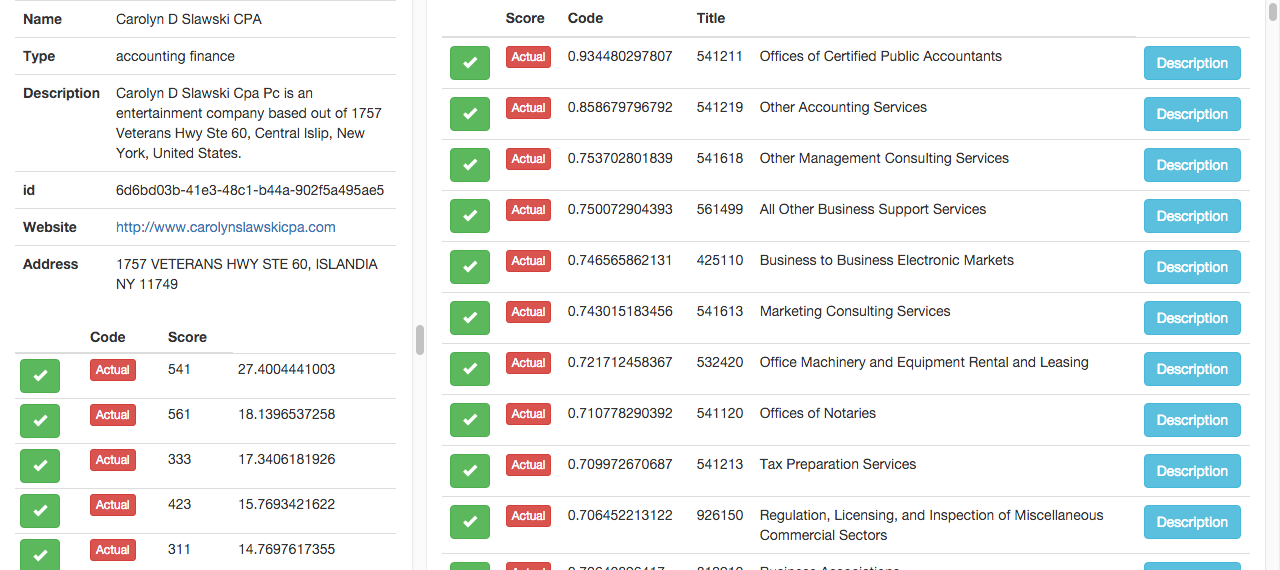
\includegraphics[width=0.5\textwidth]{handclassifier.png}

\section*{Figure 2}
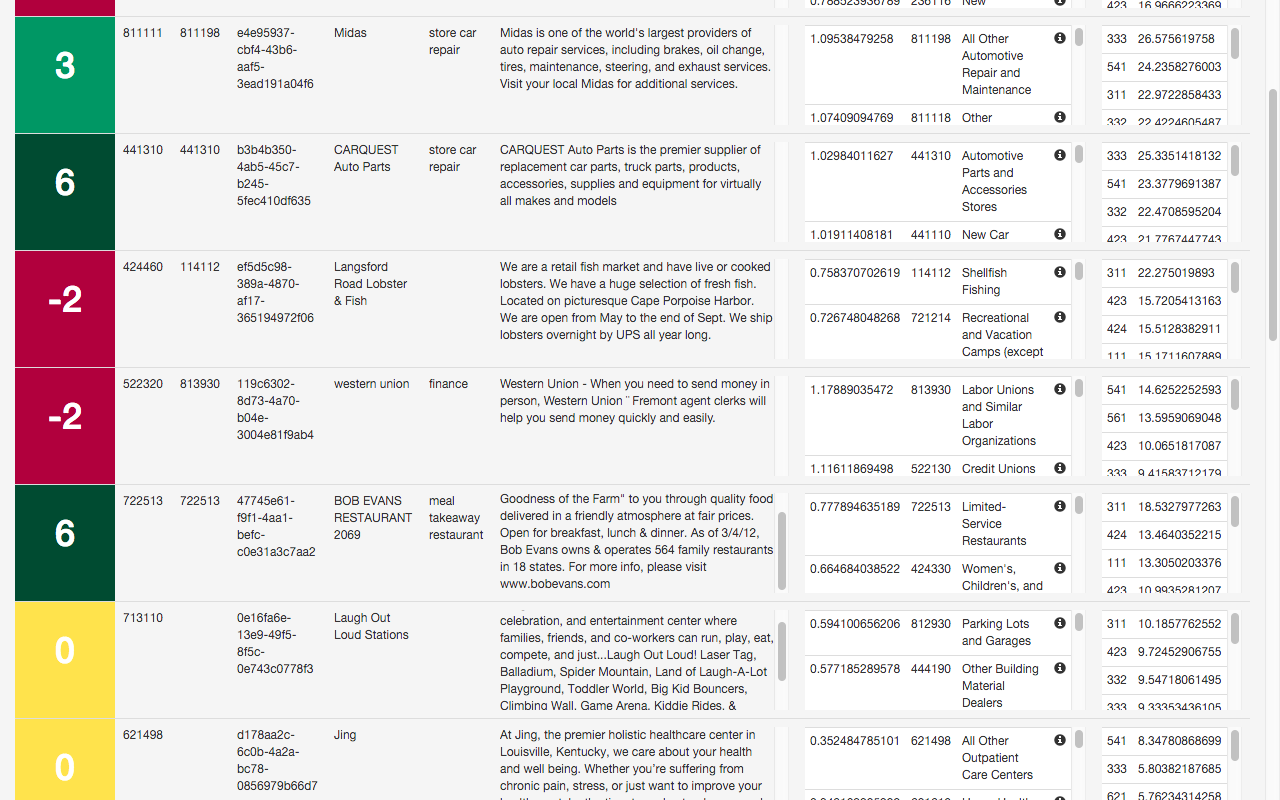
\includegraphics[width=0.5\textwidth]{database.png}

\section*{List 1}
\begin{itemize}
\item get\_business\_latlot.py: generates id\_to\_loc.pickle
\item get\_business\_types.py: generates business\_types.pickle
\item get\_naics\_data.py: generates naics\_list.json
\end{itemize}

\end{document}
